\documentclass{beamer}
\usepackage{beamerthemeOerestad}
\usetheme{Oerestad}

\usepackage[utf8]{inputenc}
\usepackage{amsfonts}
\usepackage{amsmath}
\usepackage{booktabs}
\usepackage{color}
\usepackage{colortbl}
\usepackage{dirtytalk}
\usepackage{graphicx}
\usepackage{hyperref}
\usepackage{listings}
\usepackage[square,sort,comma,numbers]{natbib}
\usepackage{url}
\usepackage{semantic}
\usepackage{tikz}
\usepackage{todonotes}

\hypersetup{
  colorlinks=true,
  urlcolor=cyan
}

\lstdefinestyle{Racket}{
  language=Lisp,
  basicstyle=\ttfamily,
  otherkeywords={\#lang,define,match,let,let*,:,->,lambda,struct,define-type,car,cdr},
  identifierstyle=\color{pink!60!blue},
  keywordstyle=\color{blue!50!black},
  stringstyle=\color{green!50!black},
  commentstyle=\color{pink!60!black}
}

\lstdefinestyle{Java}{
  language=Java,
  basicstyle=\ttfamily
}

\lstset{
  style=Racket
}

\usetikzlibrary{shapes}
\tikzstyle{element} = [text centered, node distance=1.2cm]
\tikzstyle{line} = [-, draw]

\title{Parallel Computations\\ on\\ Immutable Data Structures}
\author{Florian Biermann \\\small{\texttt{fbie@itu.dk}} \\~}

\institute{IT University of Copenhagen \& UCAS}

\date{2016-06-02}

\begin{document}

\begin{frame}
  \titlepage{}
\end{frame}

\begin{frame}[fragile]{A Recursive Function}
  \begin{center}
    $\sum_{i=1}^6 i$ ~ = ~ \lstinline{(+ 1 (+ 2 (+ 3 (+ 4 (+ 5 6)))))}
  \end{center}

  \pause{} \vspace{.5cm}

  The expression's call-tree:

  \begin{center}
    \begin{tikzpicture}[level distance=0.5cm]
      \node {\lstinline{+}}
        child {node {\lstinline{1}}}
        child {node {\lstinline{+}}
          child {node {\lstinline{2}}}
          child {node {\lstinline{+}}
            child {node {\lstinline{3}}}
            child {node {\lstinline{+}}
              child {node {\lstinline{4}}}
              child {node {\lstinline{+}}
                child {node {\lstinline{5}}}
                child {node {\lstinline{6}}}}}}};
    \end{tikzpicture}
  \end{center}
\end{frame}

\begin{frame}[fragile]{What Is The Problem?}
All operations are performed sequentially, even though it would be perfectly ok to compute

\begin{lstlisting}
  (+ 1 (+ 2 3))
\end{lstlisting}

and

\begin{lstlisting}
  (+ 4 (+ 5 6))
\end{lstlisting}

in parallel.

\pause{} \vspace{1cm}

We can re-formulate the expression and obtain the same result!
\end{frame}

\begin{frame}[fragile]{A Parallel Expression}
  \begin{center}
    $\sum_{i=1}^6 i$ ~ = ~ \lstinline{(+ (+ 1 (+ 2 3)) (+ 4 (+ 5 6)))}
  \end{center}

  \pause{} \vspace{.5cm}

  The expression's call-tree:

  \begin{center}
    \begin{tikzpicture}[level distance=.5cm]
      \tikzstyle{level 1}=[sibling distance=4.8cm]
      \tikzstyle{level 2}=[sibling distance=2.4cm]
      \tikzstyle{level 3}=[sibling distance=2.4cm]
      \node {\lstinline{+}}
        child {node {\lstinline{+}}
          child {node {\lstinline{1}}}
          child {node {\lstinline{+}}
            child {node {\lstinline{2}}}
            child {node {\lstinline{3}}}
          }
        }
        child {node {\lstinline{+}}
          child {node {\lstinline{4}}}
          child {node {\lstinline{+}}
            child {node {\lstinline{5}}}
            child {node {\lstinline{6}}}
          }
        };
    \end{tikzpicture}
  \end{center}

\pause{}

Why is this possible? Because + is an associative operation!

\begin{center}
\lstinline{(+ x (+ y z))} = \lstinline{(+ (+ x y) z)}
\end{center}
\end{frame}

\begin{frame}[fragile]{Generalizing Parallel Expressions}
We can do this for any function \lstinline{f} iff
  \begin{center}
    \lstinline{(f a (f b c))} ~ = ~ \lstinline{(f (f a b) c)}

    \vspace{1cm}

    \begin{tikzpicture}[level distance=.5cm]
      \tikzstyle{level 1}=[sibling distance=4.8cm]
      \tikzstyle{level 2}=[sibling distance=2.4cm]
      \tikzstyle{level 3}=[sibling distance=1.2cm]
      \node {\lstinline{f}}
        child {node {\lstinline{f}}
          child {node {\lstinline{f}}
            child {node {\dots}}
            child {node {\dots}}
          }
          child {node {\lstinline{f}}
            child {node {\dots}}
            child {node {\dots}}
          }
        }
        child {node {\lstinline{f}}
          child {node {\lstinline{f}}
            child {node {\dots}}
            child {node {\dots}}
          }
          child {node {\lstinline{f}}
            child {node {\dots}}
            child {node {\dots}}
          }
        };
    \end{tikzpicture}
  \end{center}
\end{frame}

\begin{frame}[fragile]{Another Problem}
Mapping a function \lstinline{f} over a \lstinline{cons} list.

\begin{lstlisting}
(: seq-map (All (A B)
    (-> (-> A B) (Listof A) (Listof B))))
(define (seq-map f xs)
  (match xs
    ['() '()]
    [(cons x xs) (cons (f x) (seq-map f xs))]))
\end{lstlisting}

\pause{} \vspace{.5cm}

Call-tree of \lstinline{seq-map}:

  \begin{center}
    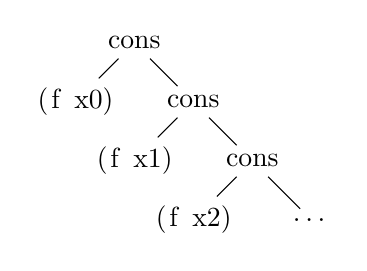
\begin{tikzpicture}[level distance=0.75cm]
      \node {\lstinline{cons}}
        child {node {\lstinline{(f x0)}}}
        child {node {\lstinline{cons}}
          child {node {\lstinline{(f x1)}}}
          child {node {\lstinline{cons}}
            child {node {\lstinline{(f x2)}}}
            child {node {\dots}}}};
    \end{tikzpicture}
  \end{center}
\end{frame}

\begin{frame}{What Is The Problem?}
  \lstinline{seq-map} is not the problem. It is the only way to handle a \lstinline{cons} list. \textbf{The real problem is the single-linked list!} It is inherently sequential.

\pause{} \vspace{1cm}

All parallel expressions we saw so far were trees. Maybe we can develop a tree data structure that we can use to implement a parallel version of \lstinline{map}?
\end{frame}

\begin{frame}[fragile]{A New Parallel Data Type}
We represent the list as a tree instead:
\begin{lstlisting}
(define-type (CatListof A) (U (leaf A) (cat A)))
(struct (A) leaf ([a : A]))
(struct (A) cat ([l : (CatListof A)]
                 [r : (CatListof A)]))
\end{lstlisting}

\pause{} \vspace{.5cm}

\lstinline{(leaf a)} produces a singleton \lstinline{CatList}.

\lstinline{(cat l r)} concatenates two \lstinline{CatList} instances.
\end{frame}

\begin{frame}[fragile]{Let's Implement Map!}
\begin{lstlisting}
(: par-map (All (A B)
  (-> (-> A B) (CatListof A) (CatListof B))))
(define (par-map f xs)
  (match xs
    [(leaf x) (leaf (f x))]
    [(cat l r) (cat (par-map f l)
                    (par-map f r))]))
\end{lstlisting}

This function is not truly parallel yet. That is the next step!

\end{frame}

\begin{frame}[fragile]{Parallelism in Racket}
In Racket we use a fork/join style model of parallel computations. Fork is called \lstinline{future} and join is called \lstinline{touch}:

\begin{lstlisting}
(: in-parallel (All (A B C)
  (-> (-> A B) (-> A C) A (Pairof B C))))
(define (in-parallel f g x)
  (let ([fx (future (lambda () (f x)))]
        [gx (g x)])
    (cons (touch fx) gx)))
\end{lstlisting}

\pause{} \vspace{.5cm}

Racket has a built-in scheduler for \lstinline{future}s, so we give a lot of control to the run-time.

\lstinline{(: future (All (A) (-> (-> A) (Futureof A))))}

\lstinline{(: touch  (All (A) (-> (Futureof A) A)))}
\end{frame}

\begin{frame}[fragile]{Parallelizing Map, For Real}
\begin{lstlisting}
(: par-map (All (A B)
  (-> (-> A B) (CatListof A) (CatListof B))))
(define (par-map f xs)
  (match xs
    [(leaf x) (leaf (f x))]
    [(cat l r)
       (let ([l0 (future ;; Map l in parallel.
                   (lambda () (par-map f l)))]
             [r0 (future ;; Map r in parallel.
                   (lambda () (par-map f r)))])
         (cat (touch l0) (touch r0)))]))
\end{lstlisting}

The recursive call is wrapped in a \lstinline{future}!
\end{frame}

\begin{frame}{Pro and Contra}
  The good parts:

  \begin{itemize}
  \item The build-in scheduler decides on the number of threads to use.
  \item A thread that is blocked by \lstinline{touch} is de-scheduled until the \lstinline{touch}ed \lstinline{future} is done, no locking, spinning etc.
  \item As a result, we do not have to manually decide \textbf{how} to split up work across hardware threads.
  \end{itemize}

  \pause{}

  The bad parts:
  \begin{itemize}
  \item A list has $O(n)$ memory overhead, a tree $O(n \log n)$.
  \item If the tree is not balanced, we lose parallelism -- mitigate by balancing algorithm!
  \item Maybe we spawn \textbf{excessively many futures} and put too much strain on the scheduler?
  \end{itemize}
\end{frame}

\begin{frame}[fragile]{An Improved Variant}
If the size of the tree is too small, then the overhead of constructing \lstinline{future}s dominates the run-time cost. We can handle this problem by using lists as leaves instead of scalar values.

\vspace{0.5cm}

We call such a tree a \textbf{Rope}:

\begin{lstlisting}
(define-type (Ropeof A) (U (Leaf A) (Cat A)))
(struct (A) Leaf ([as : (Listof A)]))
(struct (A) Cat  ([l  : (Ropeof A)]
                  [r  : (Ropeof A)]))
\end{lstlisting}
\end{frame}

\begin{frame}{Ropes: Trees With Lists as Leaves}
  We must define a \textbf{maximum size} $s_{\max}$ for leaves. In this example, $s_{\max}\,=\,3$:

  \begin{center}
    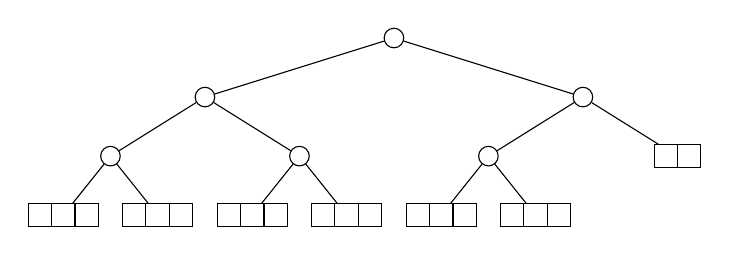
\begin{tikzpicture}[level distance=0.75cm]
      \tikzstyle{every node}=[scale=0.75]]
      \tikzstyle{level 1}=[sibling distance=4.8cm]
      \tikzstyle{level 2}=[sibling distance=2.4cm]
      \tikzstyle{level 3}=[sibling distance=1.2cm]
      \node [circle, draw] {}
        child {node [circle, draw] {}
          child {node [circle, draw] {}
            child {node [rectangle split, rectangle split horizontal, rectangle split parts=3, draw] {}}
            child {node [rectangle split, rectangle split horizontal, rectangle split parts=3, draw] {}}
          }
          child {node [circle, draw] {}
            child {node [rectangle split, rectangle split horizontal, rectangle split parts=3, draw] {}}
            child {node [rectangle split, rectangle split horizontal, rectangle split parts=3, draw] {}}
          }
        }
        child {node [circle, draw] {}
          child {node [circle, draw] {}
            child {node [rectangle split, rectangle split horizontal, rectangle split parts=3, draw] {}}
            child {node [rectangle split, rectangle split horizontal, rectangle split parts=3, draw] {}}
          }
          child {node [rectangle split, rectangle split horizontal, rectangle split parts=2, draw] {}}
        };
    \end{tikzpicture}
  \end{center}
\end{frame}

\begin{frame}[fragile]{New Syntax: Recursive Let}

Standard \lstinline{let}:
\begin{lstlisting}
(let ([x 1]
      [y (+ 2 x)])
  (* y x))
\end{lstlisting}

\pause{} \vspace{0.25cm}

\textcolor{red}{\texttt{Undefined identifier: x}}

\pause{} \vspace{0.5cm}

Solution: \lstinline{let*}, recursive let-binding:

\begin{lstlisting}
(let* ([x 1]
       [y (+ 2 x)])
  (* y x))
\end{lstlisting}

Allows bindings to reference one-another.
\end{frame}

\end{document}
